%----------------------------------------------------------------------------------------
%	PACKAGES AND OTHER DOCUMENT CONFIGURATIONS
%----------------------------------------------------------------------------------------

\documentclass[paper=a4, fontsize=11pt]{scrartcl} % A4 paper and 11pt font size

\usepackage[T1]{fontenc} % Use 8-bit encoding that has 256 glyphs
\usepackage{fourier} % Use the Adobe Utopia font for the document - comment this line to return to the LaTeX default
\usepackage[english]{babel} % English language/hyphenation
\usepackage{amsmath,amsfonts,amsthm, amssymb} % Math packages
\usepackage[utf8]{inputenc}

\usepackage{graphicx}
\usepackage{float}

\usepackage{lipsum} % Used for inserting dummy 'Lorem ipsum' text into the template

\usepackage{sectsty} % Allows customizing section commands
\allsectionsfont{\centering \normalfont\scshape} % Make all sections centered, the default font and small caps

\usepackage{fancyhdr} % Custom headers and footers
\pagestyle{fancyplain} % Makes all pages in the document conform to the custom headers and footers
\fancyhead{} % No page header - if you want one, create it in the same way as the footers below
\fancyfoot[L]{} % Empty left footer
\fancyfoot[C]{} % Empty center footer
\fancyfoot[R]{\thepage} % Page numbering for right footer
\renewcommand{\headrulewidth}{0pt} % Remove header underlines
\renewcommand{\footrulewidth}{0pt} % Remove footer underlines
\setlength{\headheight}{13.6pt} % Customize the height of the header

\numberwithin{equation}{section} % Number equations within sections (i.e. 1.1, 1.2, 2.1, 2.2 instead of 1, 2, 3, 4)
\numberwithin{figure}{section} % Number figures within sections (i.e. 1.1, 1.2, 2.1, 2.2 instead of 1, 2, 3, 4)
\numberwithin{table}{section} % Number tables within sections (i.e. 1.1, 1.2, 2.1, 2.2 instead of 1, 2, 3, 4)

\setlength\parindent{0pt} % Removes all indentation from paragraphs - comment this line for an assignment with lots of text

%----------------------------------------------------------------------------------------
%	TITLE SECTION
%----------------------------------------------------------------------------------------

\newcommand{\horrule}[1]{\rule{\linewidth}{#1}} % Create horizontal rule command with 1 argument of height

\title{	
    \normalfont \normalsize 
    \textsc{TDT4173 - Machine Learning \& Case-based Reasoning, IDI, NTNU} \\ [25pt] % Your university, school and/or department name(s)
    \horrule{0.5pt} \\[0.4cm] % Thin top horizontal rule
    \huge Problem set 4 - Theory \\ % The assignment title
    \horrule{2pt} \\[0.5cm] % Thick bottom horizontal rule
}

\author{Øyvind Robertsen} % Your name

\date{\normalsize\today} % Today's date or a custom date

\begin{document}

\maketitle % Print the title

%----------------------------------------------------------------------------------------
%	PROBLEM 1
%----------------------------------------------------------------------------------------

\section{Theory}

\subsection{Case-Based Reasoning}

\subsubsection{Characteristics}

Case-Based Reasoning bases itself upon the assumption that similar problems have similar solutions.
In CBR, we store cases, situations with corresponding solutions, in a database, and retrieve them when a new situation arises.
To know which case to retrieve, we need a metric of similarity between cases.
This is usually some approximation based on various descriptive properties of the cases.

While most machine learning approaches are trained to approximate a global target function given some problem domain, CBR systems focus on reusing solutions to problems that are similar to the one at hand.

Where other machine-learning approaches often consist of one algorithm approximating a global target function, CBR is more of a workflow.
When solving problems with a CBR system, the following steps are followed:

\begin{itemize}
    \item \textbf{Retrieving} - Find relevant/similar experience from the case base.
    \item \textbf{Reusing} - Apply (possibly adapted) solutions from the retrieved case onto the current situation.
    \item \textbf{Revising} - Evaluate how well the solution performed in the context of the current situation and revise.
    \item \textbf{Retaining} - Store the new experience in the case base.
\end{itemize}

\subsubsection{Influence from Cognitive Science}

Case-Based Reasoning attempts to model the human problem solving behaviour, by emphasizing experience over knowledge.

\subsubsection{Surface Similarity vs. Structural Similarity}

The difference between surface similarity and structural similarity lies in wether or not a feature is casually related to goal attainment.
In other words, a feature is said to be structural if it is central in determining wether or not one case is a good analogy for another.
Similarily, a surface similarity is one that is not crucial to the concept to be described.

\section{Practical}

\subsection{Case Modelling}

\begin{figure}[H]
    \centering
    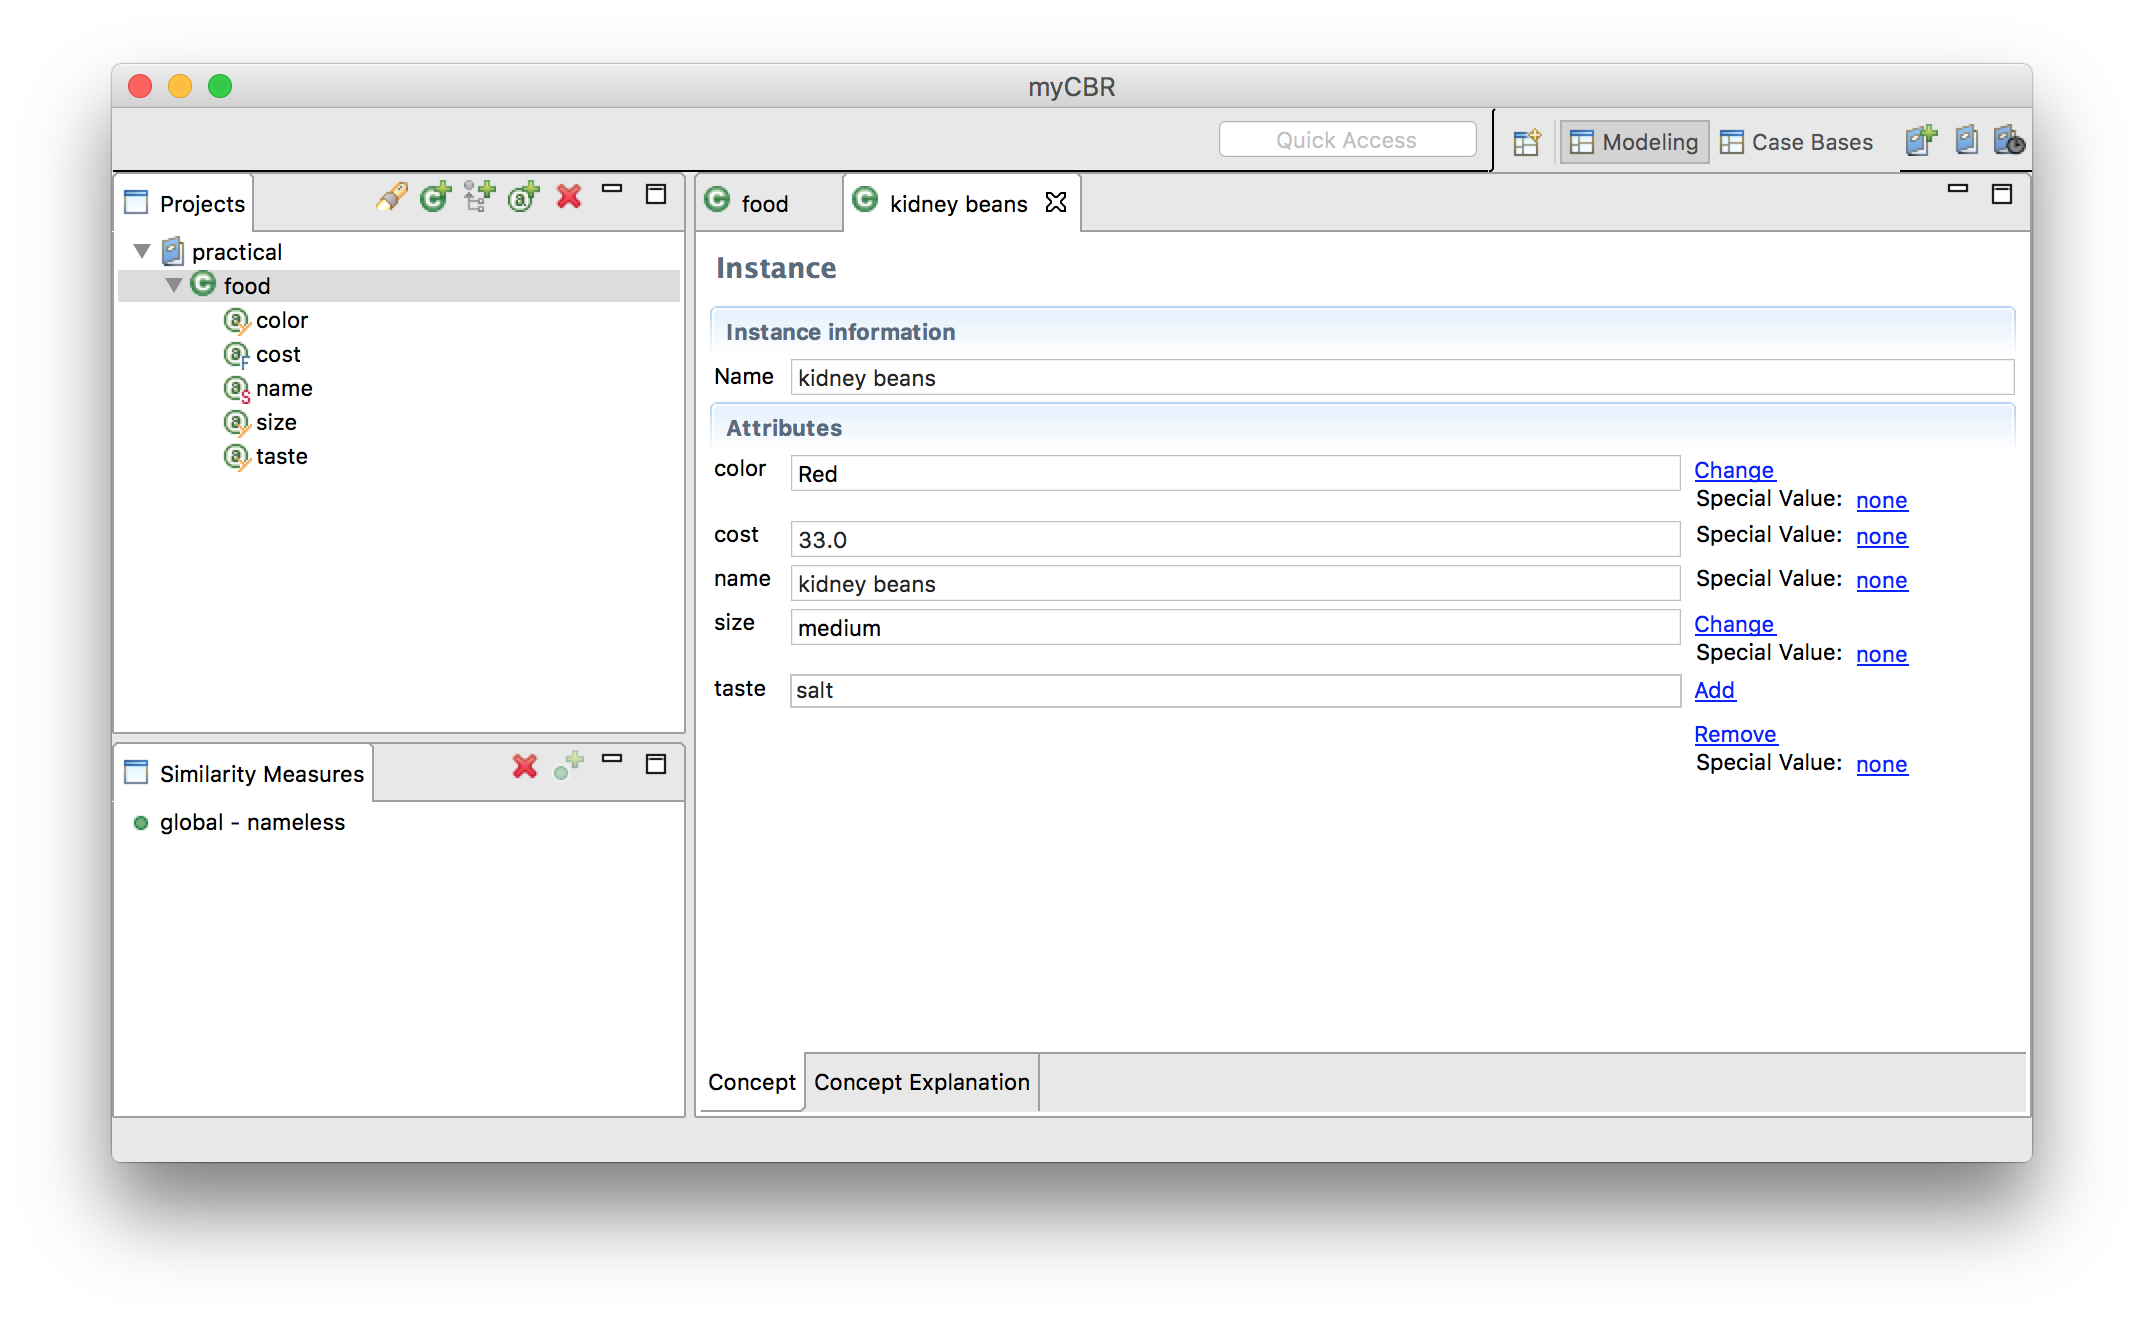
\includegraphics[width=\linewidth]{img/instance.png}
    \caption{The kidney bean instance} \label{fig:instance}
\end{figure}

\subsection{Case Retrieval}

\subsubsection{Global Similarity Measure}


\begin{figure}[H]
    \centering
    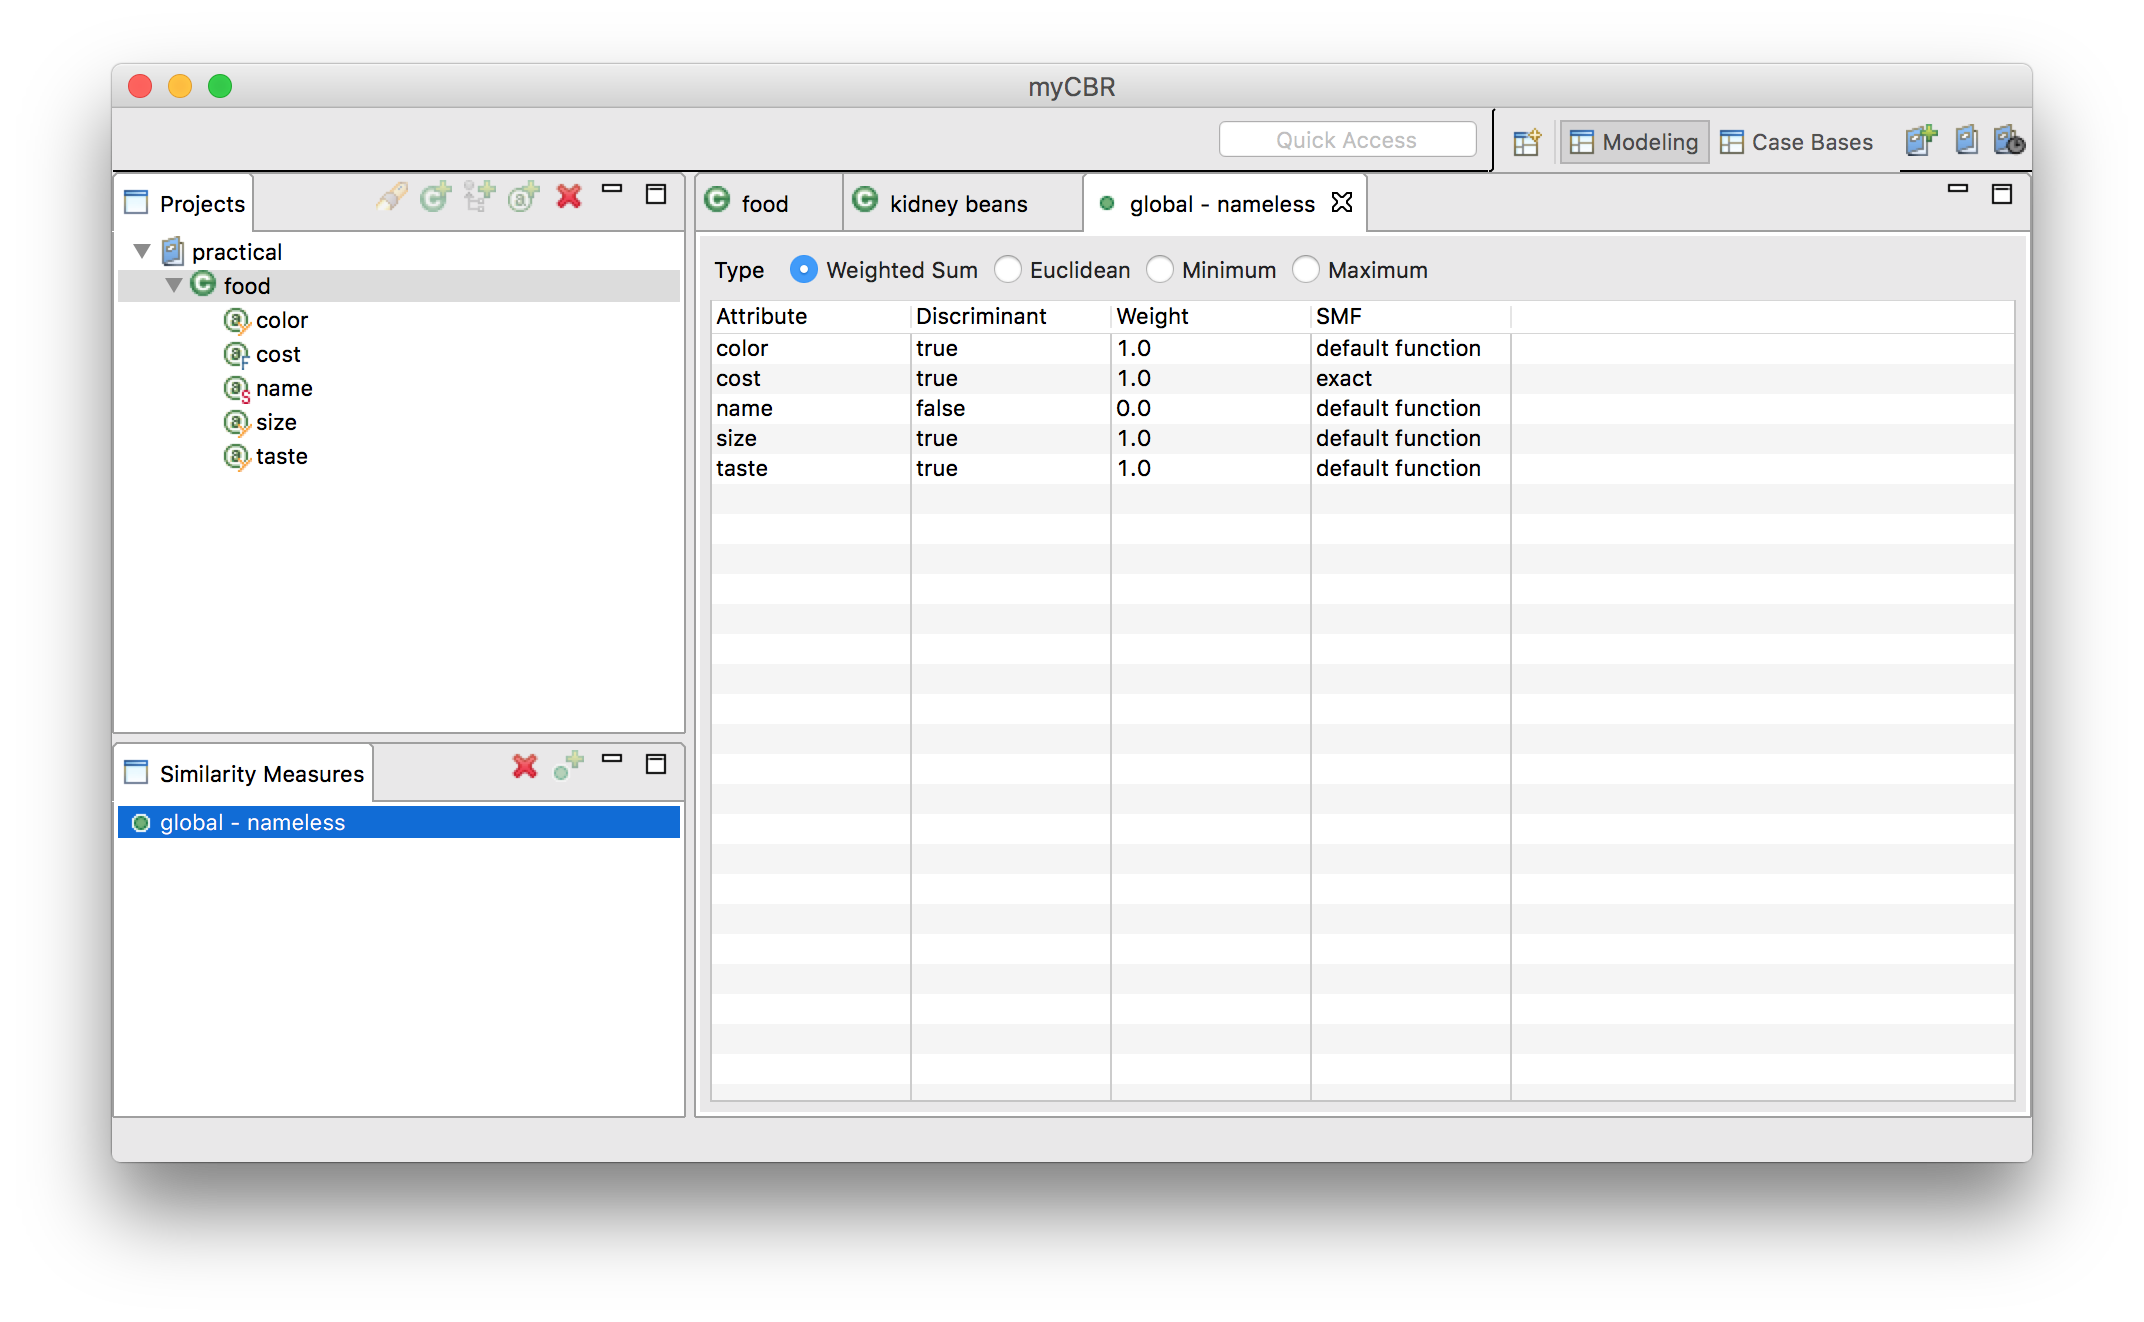
\includegraphics[width=\linewidth]{img/global.png}
    \caption{Global similarity function for the Food concept} \label{fig:global}
\end{figure}


\begin{figure}[H]
    \centering
    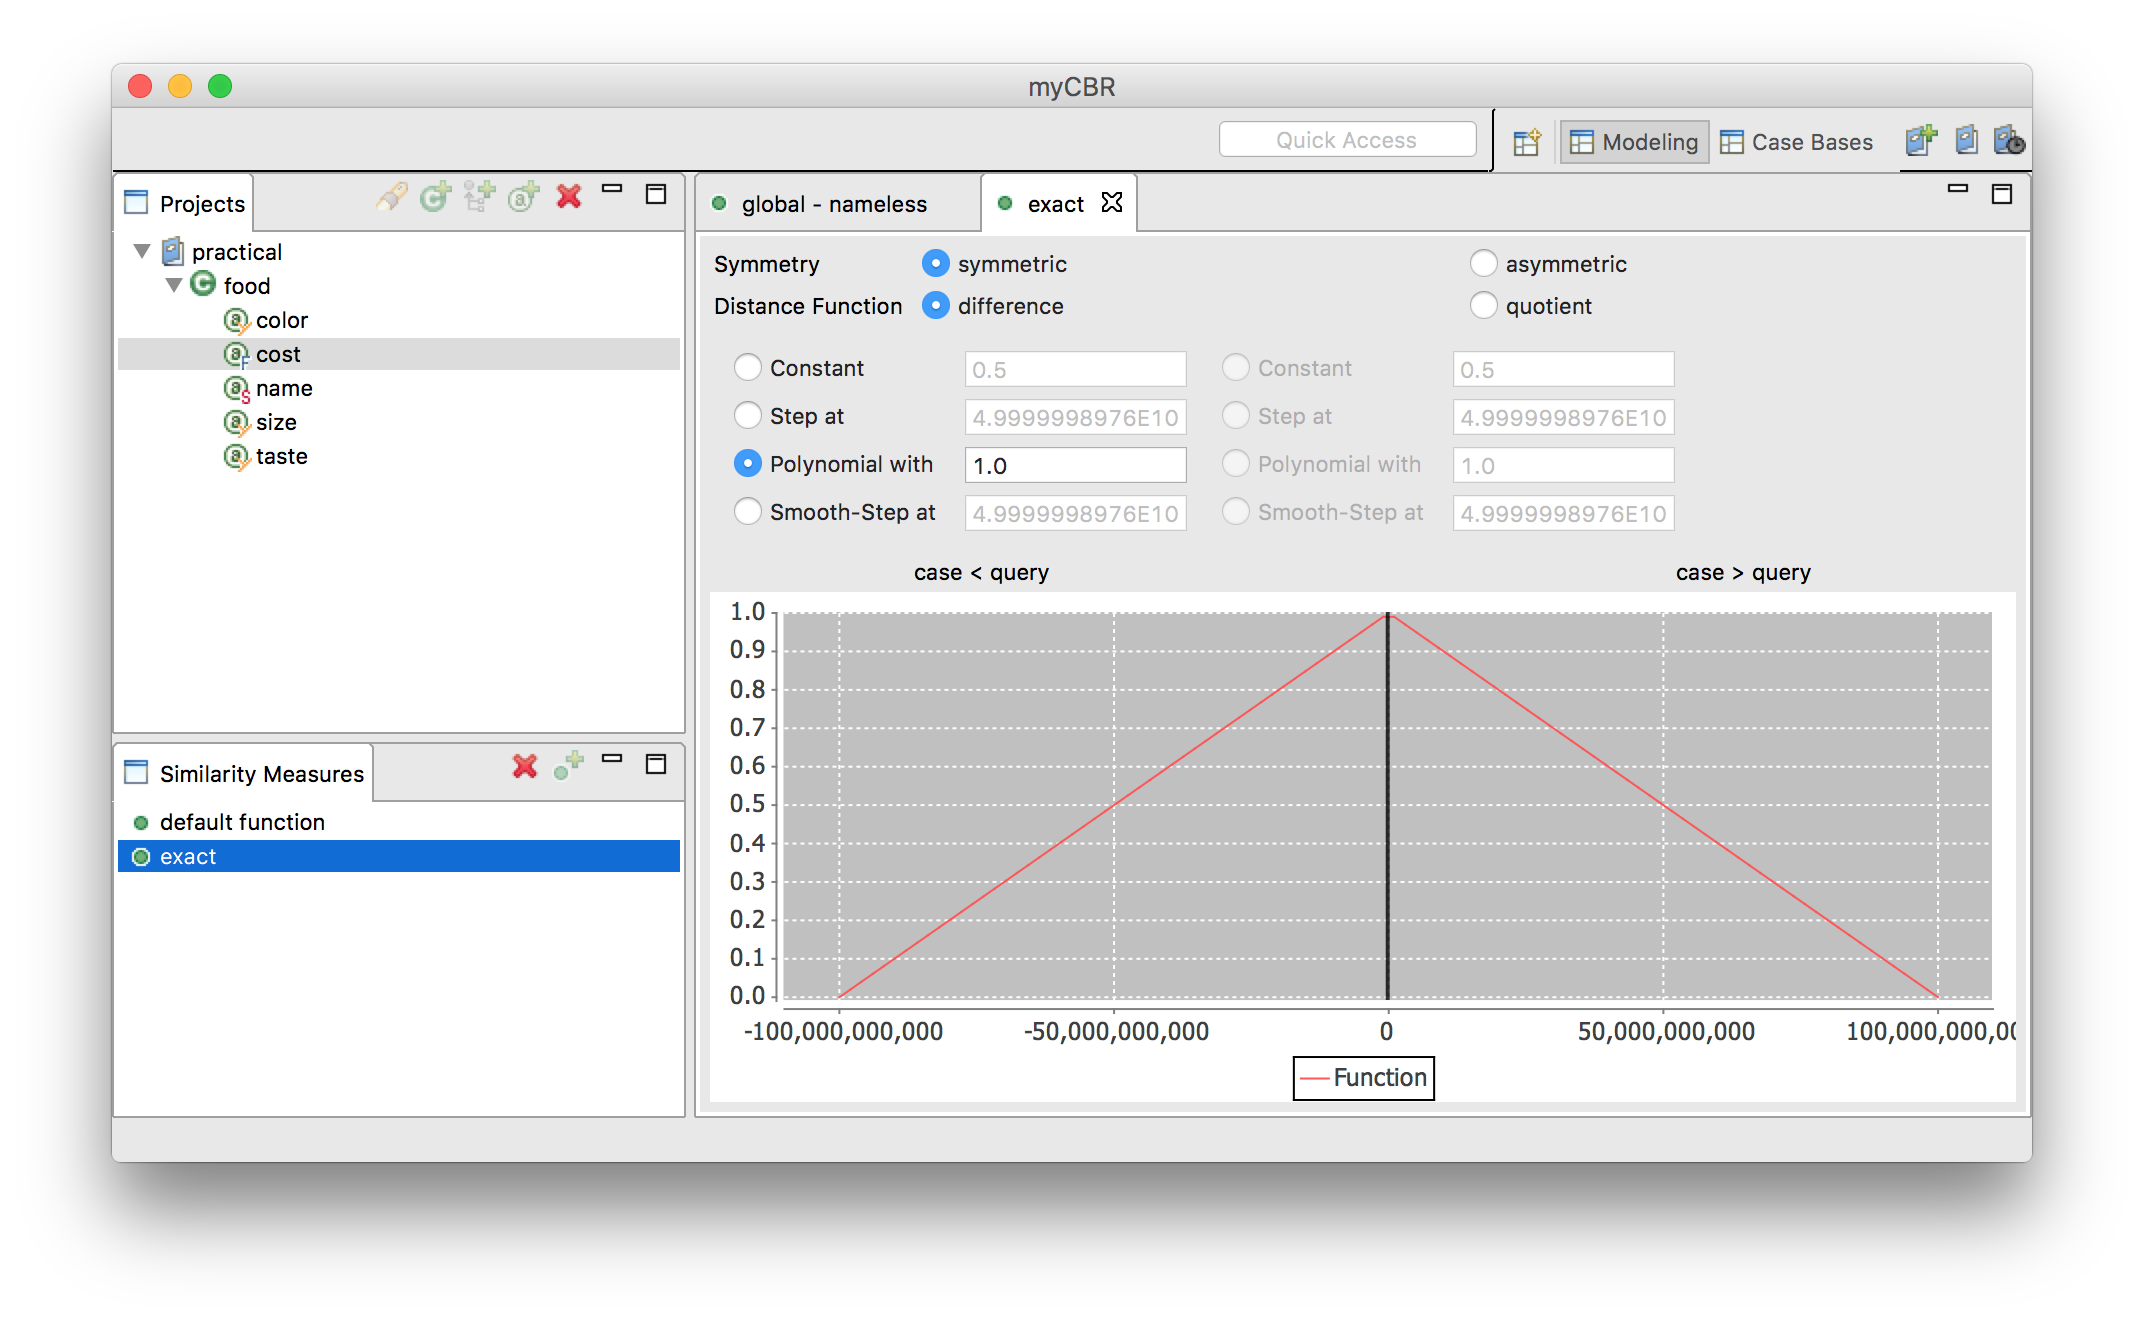
\includegraphics[width=\linewidth]{img/cost.png}
    \caption{Similarity function for the cost attribute} \label{fig:cost}
\end{figure}


\begin{figure}[h]
    \centering
    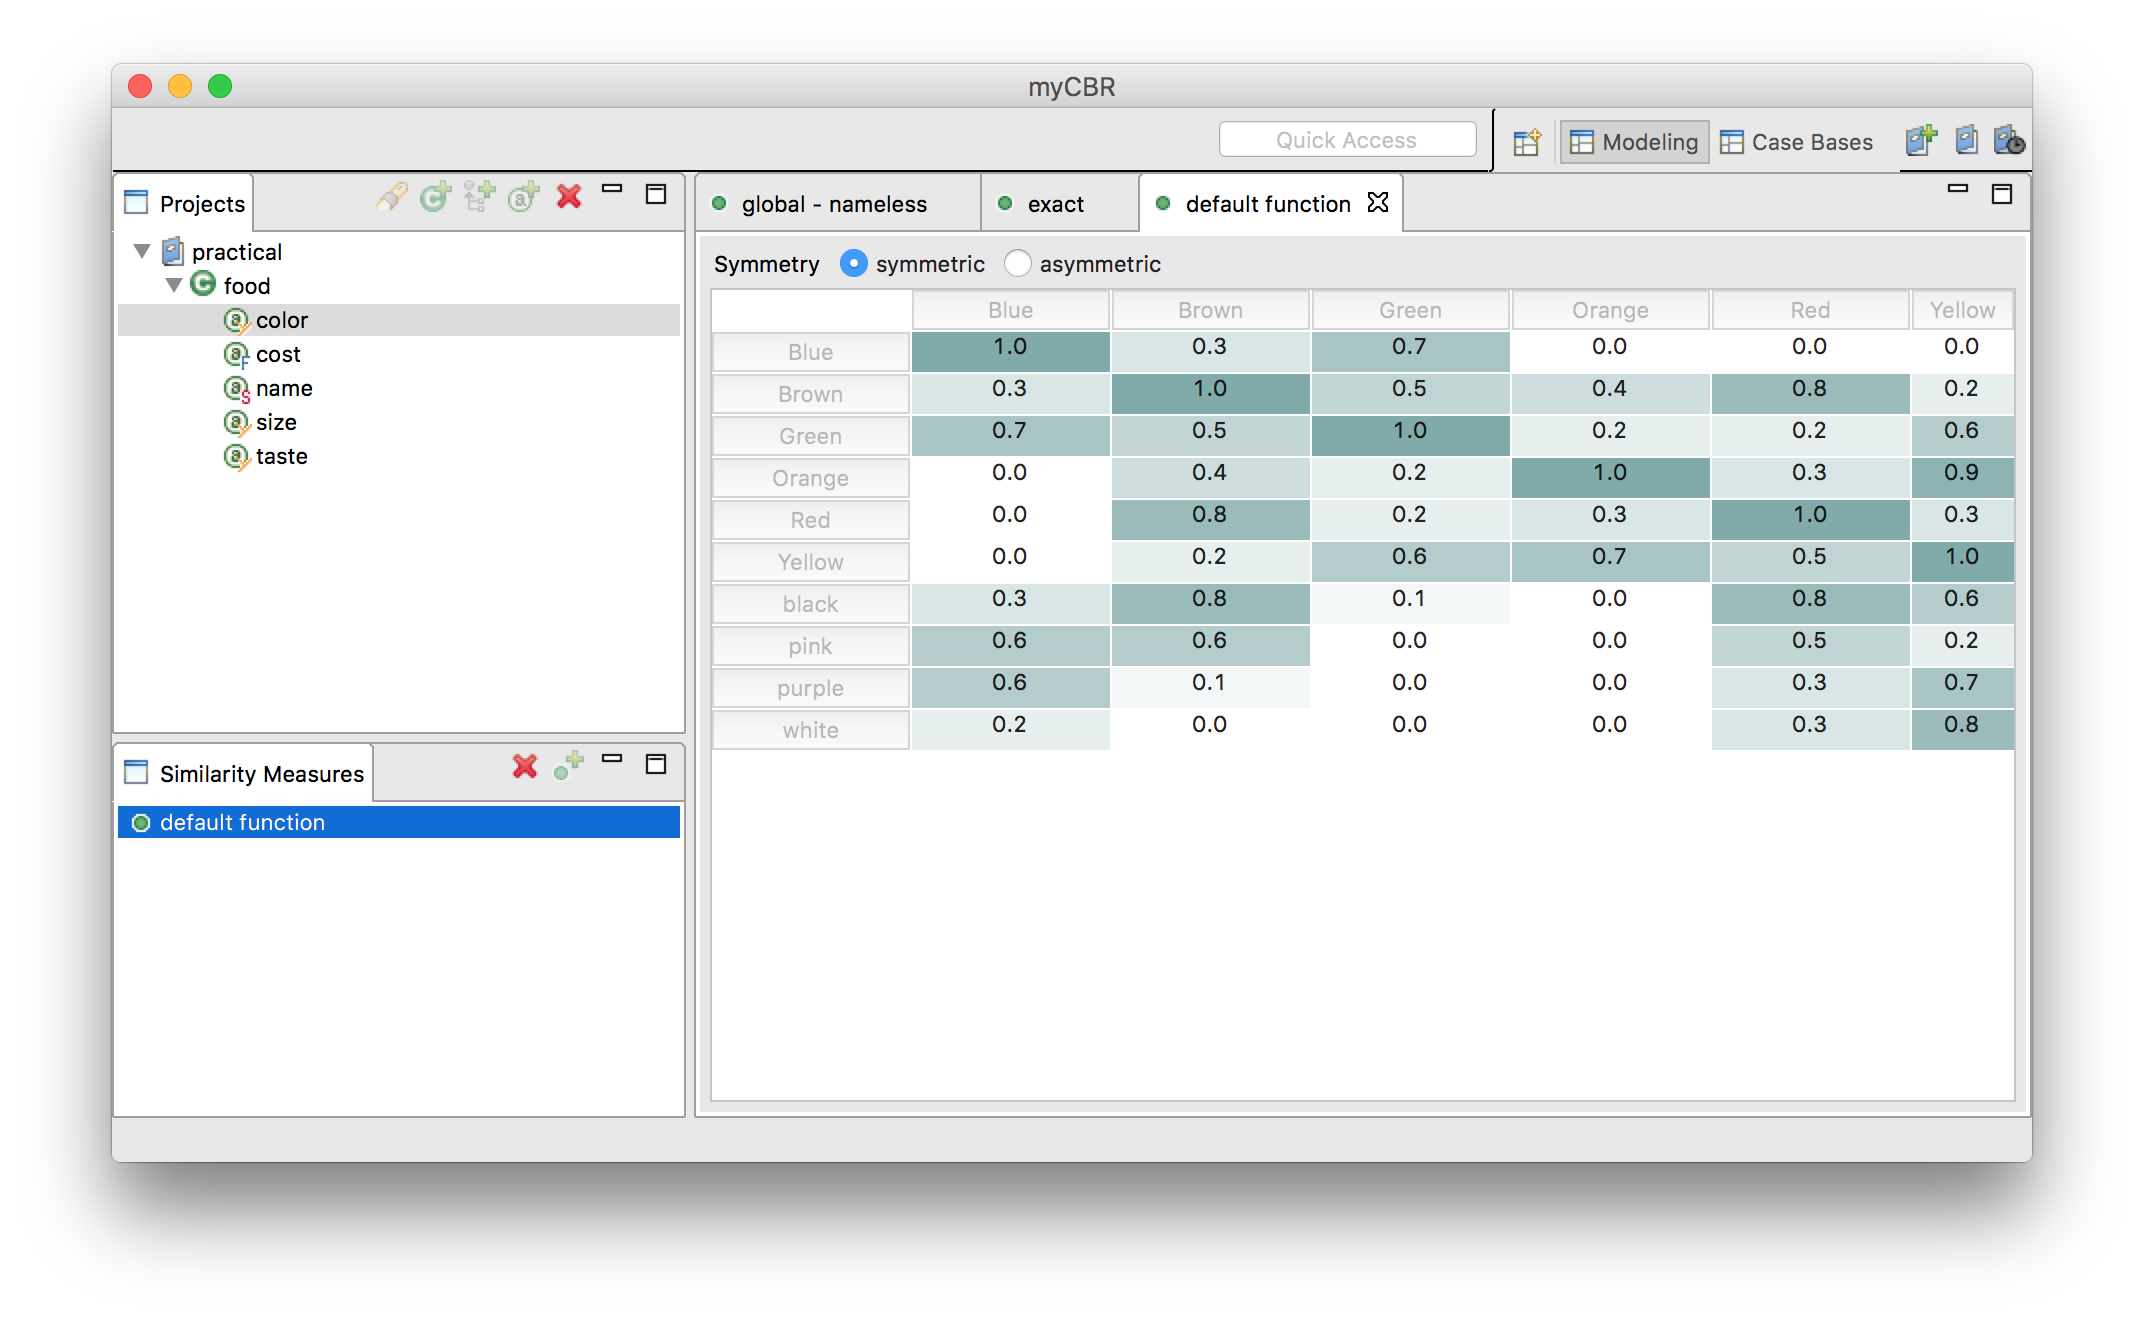
\includegraphics[width=\linewidth]{img/color.png}
    \caption{Similarity function for the color attribute} \label{fig:color}
\end{figure}


\begin{figure}[h]
    \centering
    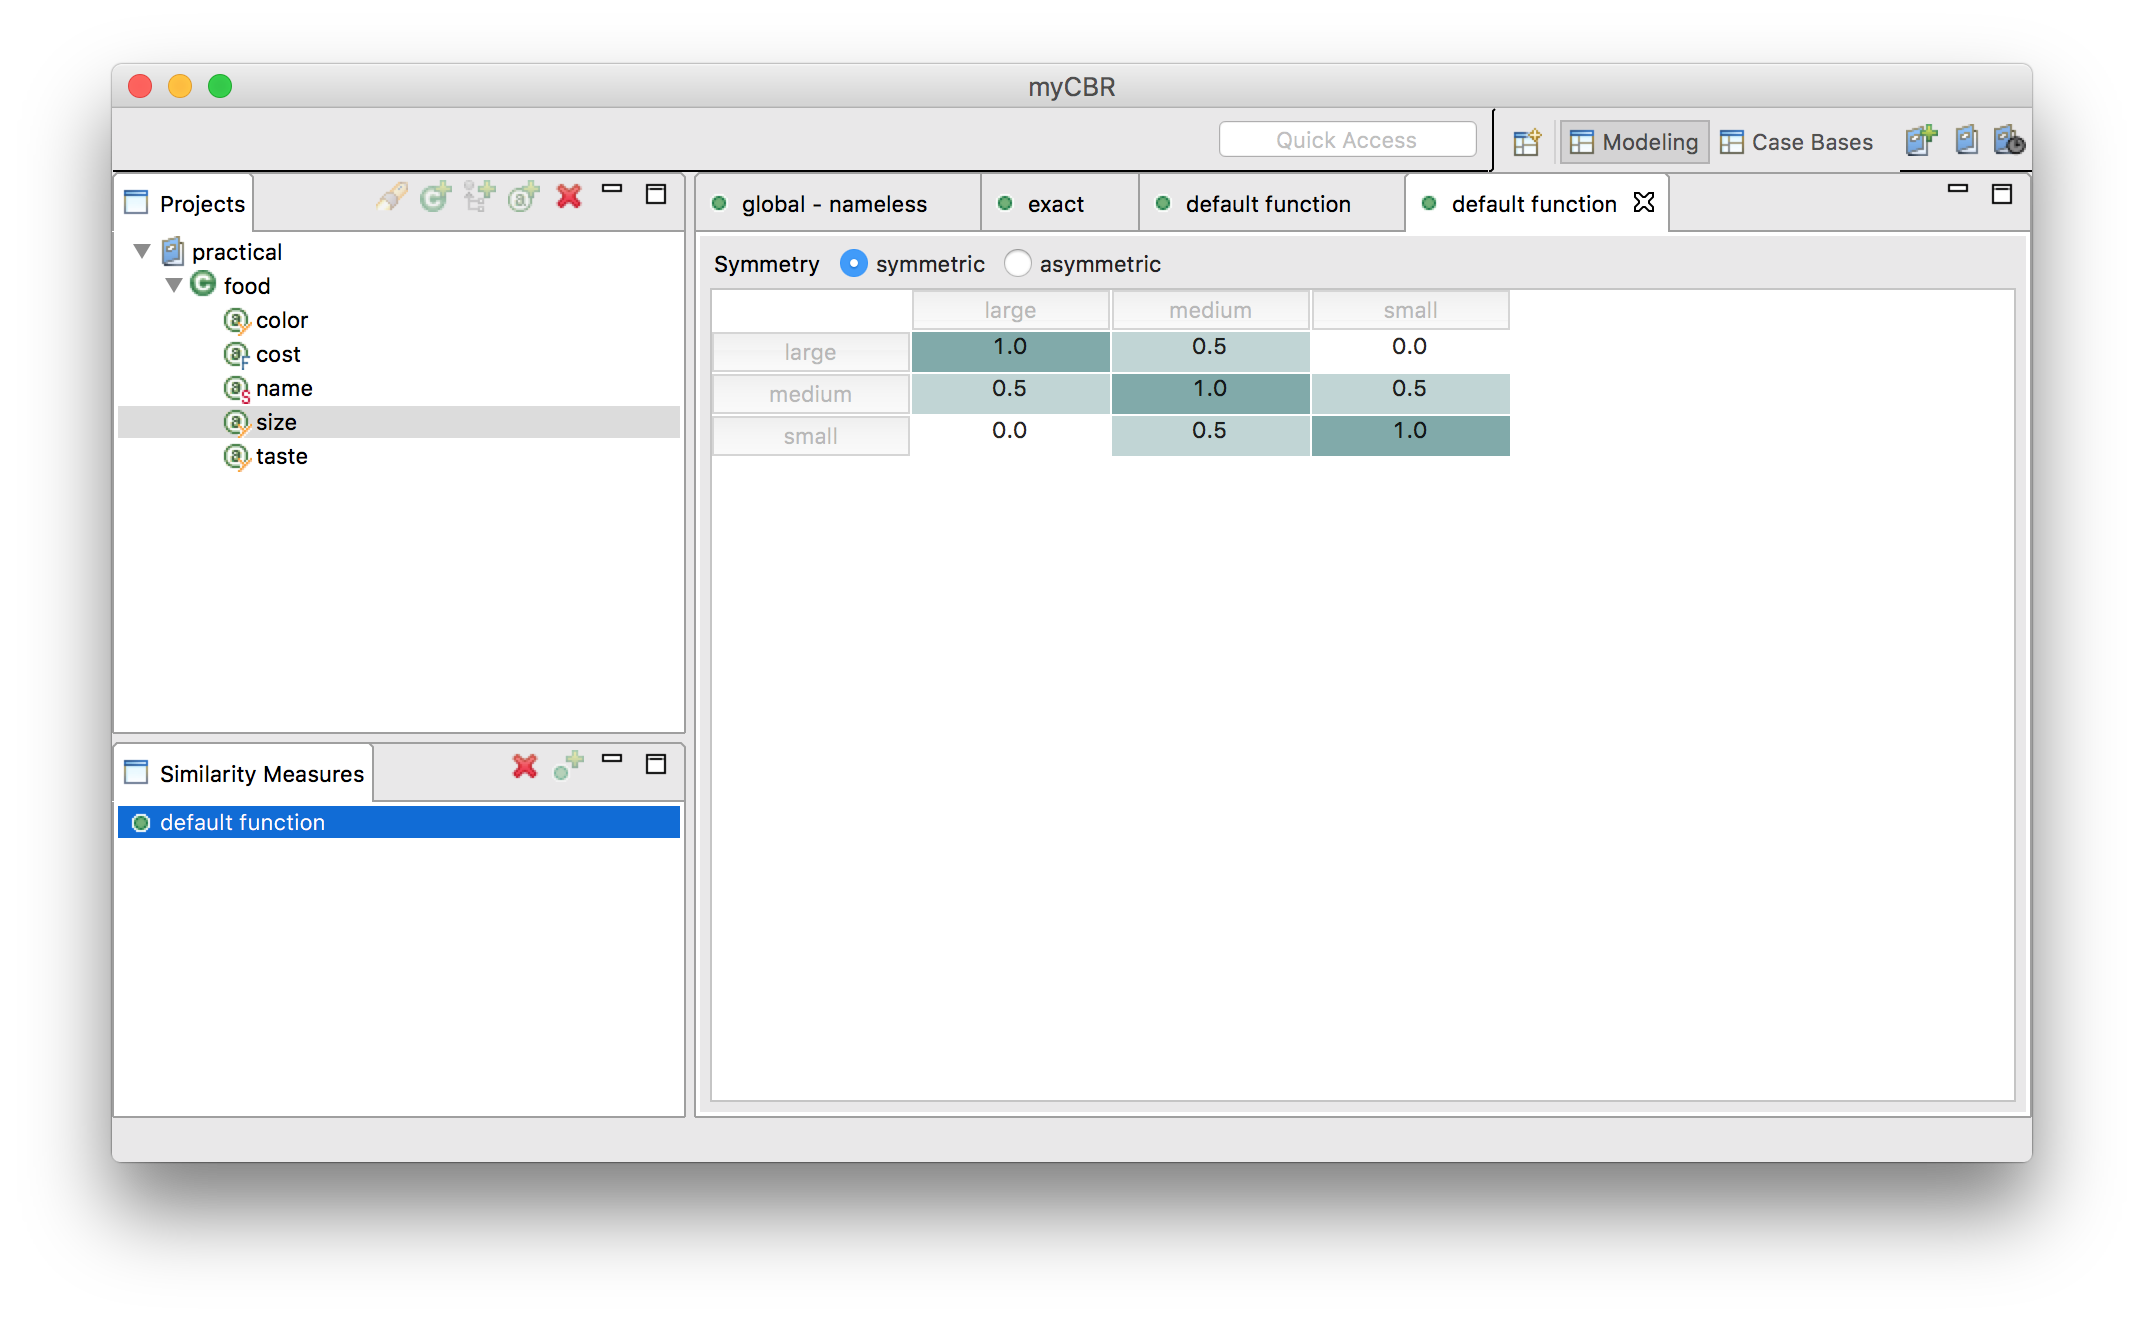
\includegraphics[width=\linewidth]{img/size.png}
    \caption{Similarity function for the size attribute} \label{fig:size}
\end{figure}

\subsubsection{Retrival}


\begin{figure}[h]
    \centering
    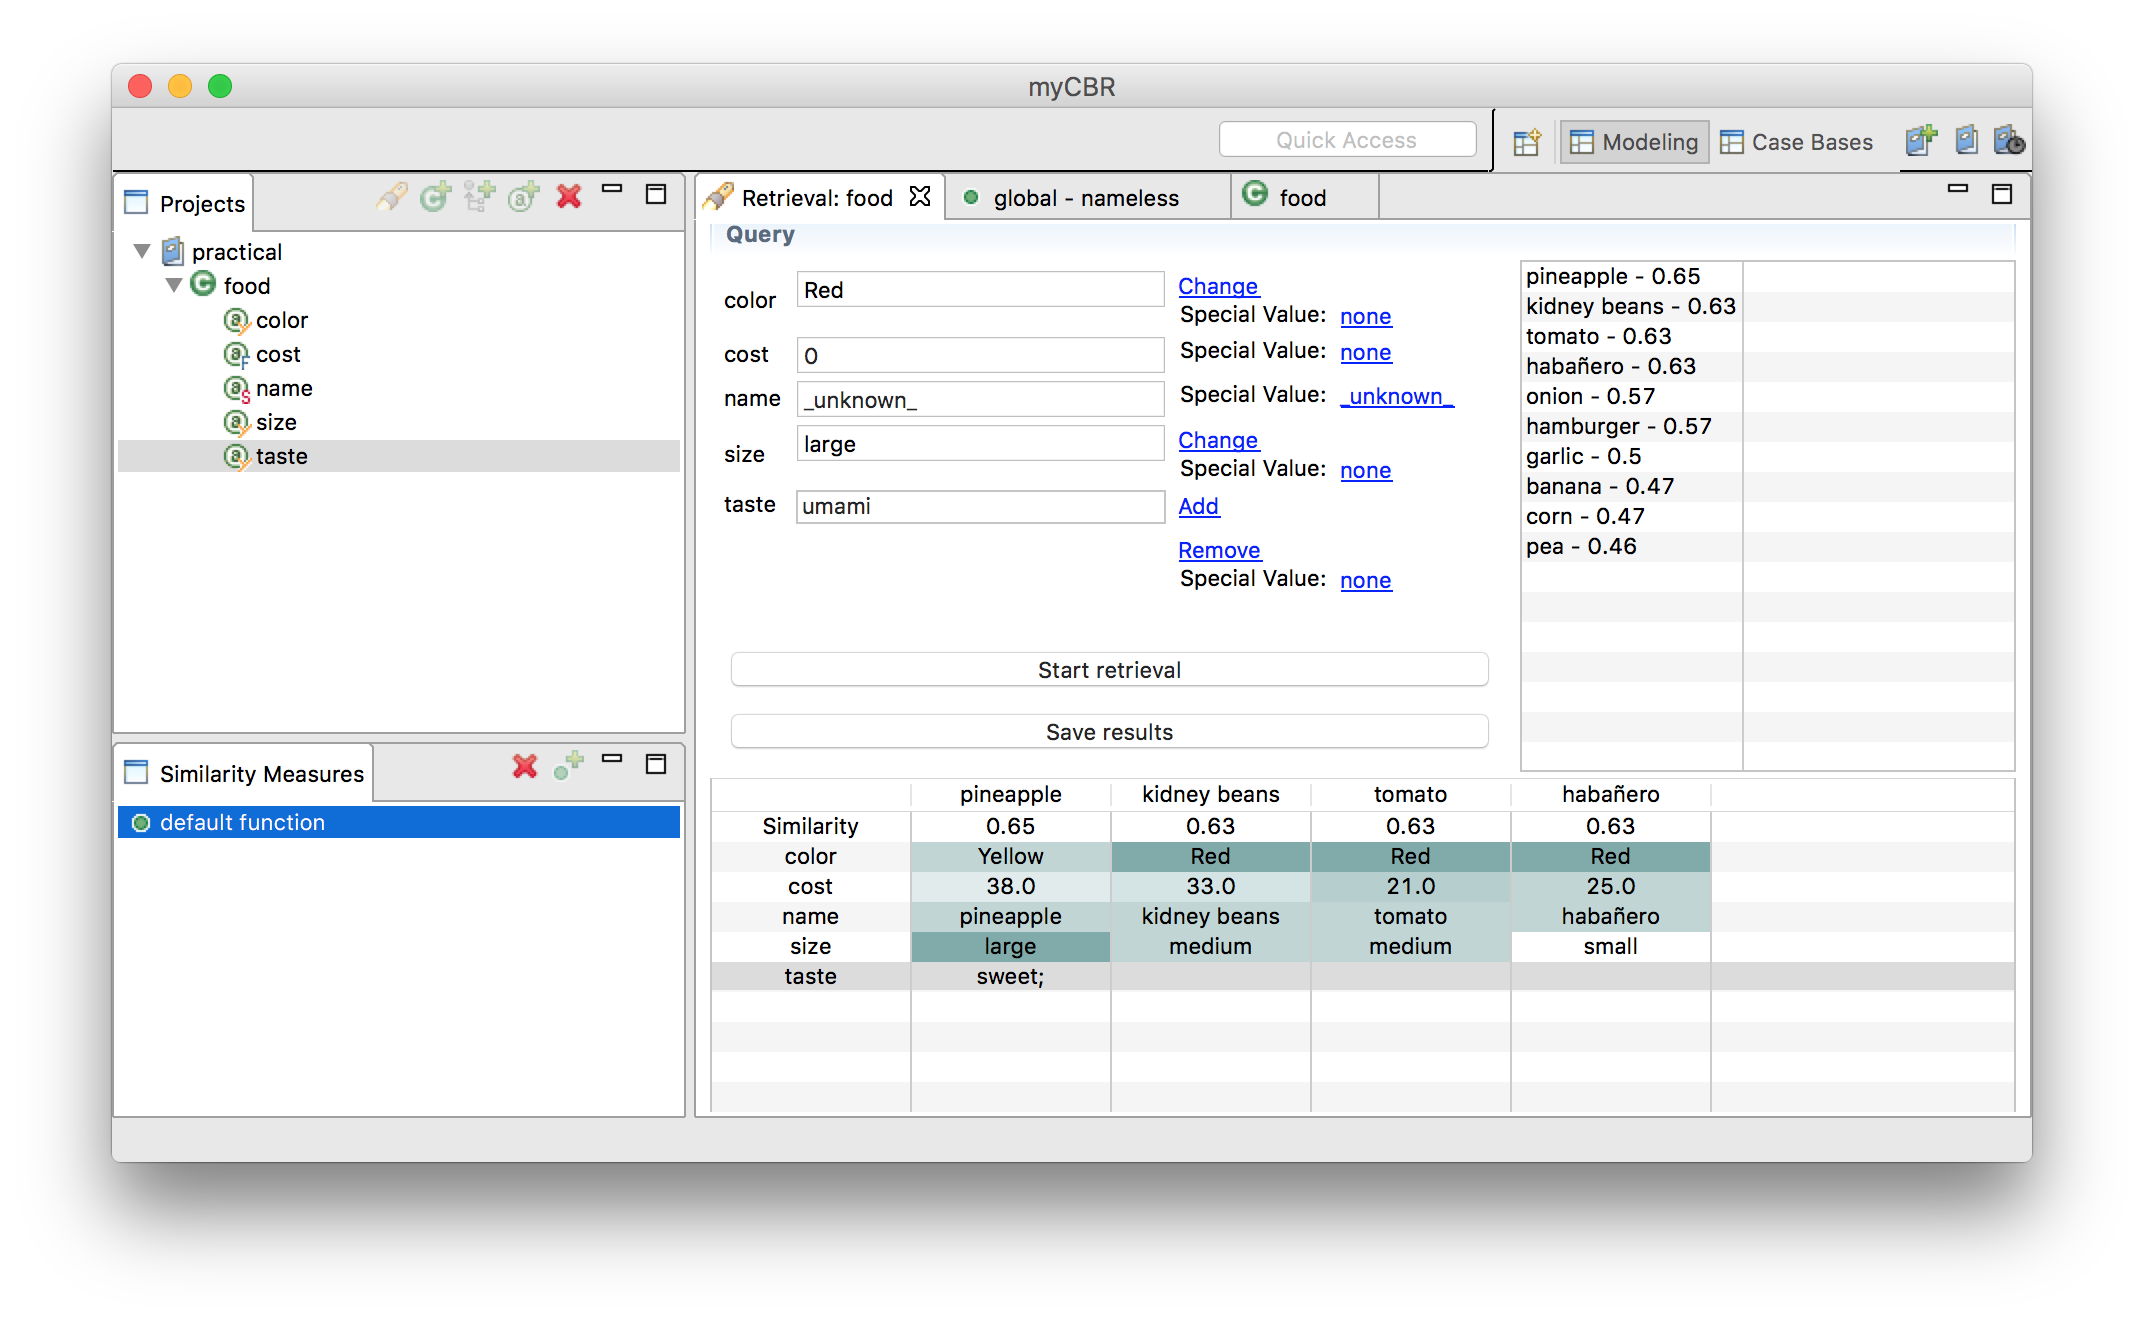
\includegraphics[width=\linewidth]{img/interesting.png}
    \caption{Interesting query} \label{fig:interesting}
\end{figure}

In the query shown in figure~\ref{fig:interesting}, I have queried the case base for cheap, red, large food that tastes umami.
None of the results are all these things, the top result isn't even red.
As for explaining the top 3 results, there really isn't much to explain.
The scores are a weighted sum of scores from subsequent similarity functions, with all weights being $1.0$.


\subsubsection{Interesting/Unexpected}

Most of the queries I performed yielded the results I expected, and as such, I have no unexpected results to show to.
As for what can potentially cause unexpected results, discriminants that are not properly weighted and similarity functions that don't account for certain cases or are not representative of the reality we want to describe, come to mind.

\subsubsection{CBR cycle}

\begin{itemize}
        \item Query for food with desired attributes, retrieve top result.
        \item Cook/eat food that is similar.
        \item Compare retrieved attributes with experience.
        \item Store experience about new food.
\end{itemize}

\end{document}

